\chapter{Tools}



\section{Web Development Languages}

\subsection{JavaScript}

\subsection{TypeScript}


\section{Native Application Development}

\subsection{Node JS}

\subsection{Python}

\subsection{C/C++}



\section{Frontend Frameworks and Libraries}

There is a wide range of available \ac{JS} frameworks to build dynamic frontends for \ac{SPA}s and \ac{PWA}s. The three libraries currently dominating the landscape are \emph{React}, developed by \emph{Facebook} in 2013, and \emph{Vue.js}, created by Evan You in 2014. These libraries can be used with frameworks to offer complete routing and state management solutions. Another popular framework is \emph{Angular}, initially released by \emph{Google} in 2010 and re-released in 2016.

\begin{figure}[h]
    \centering
    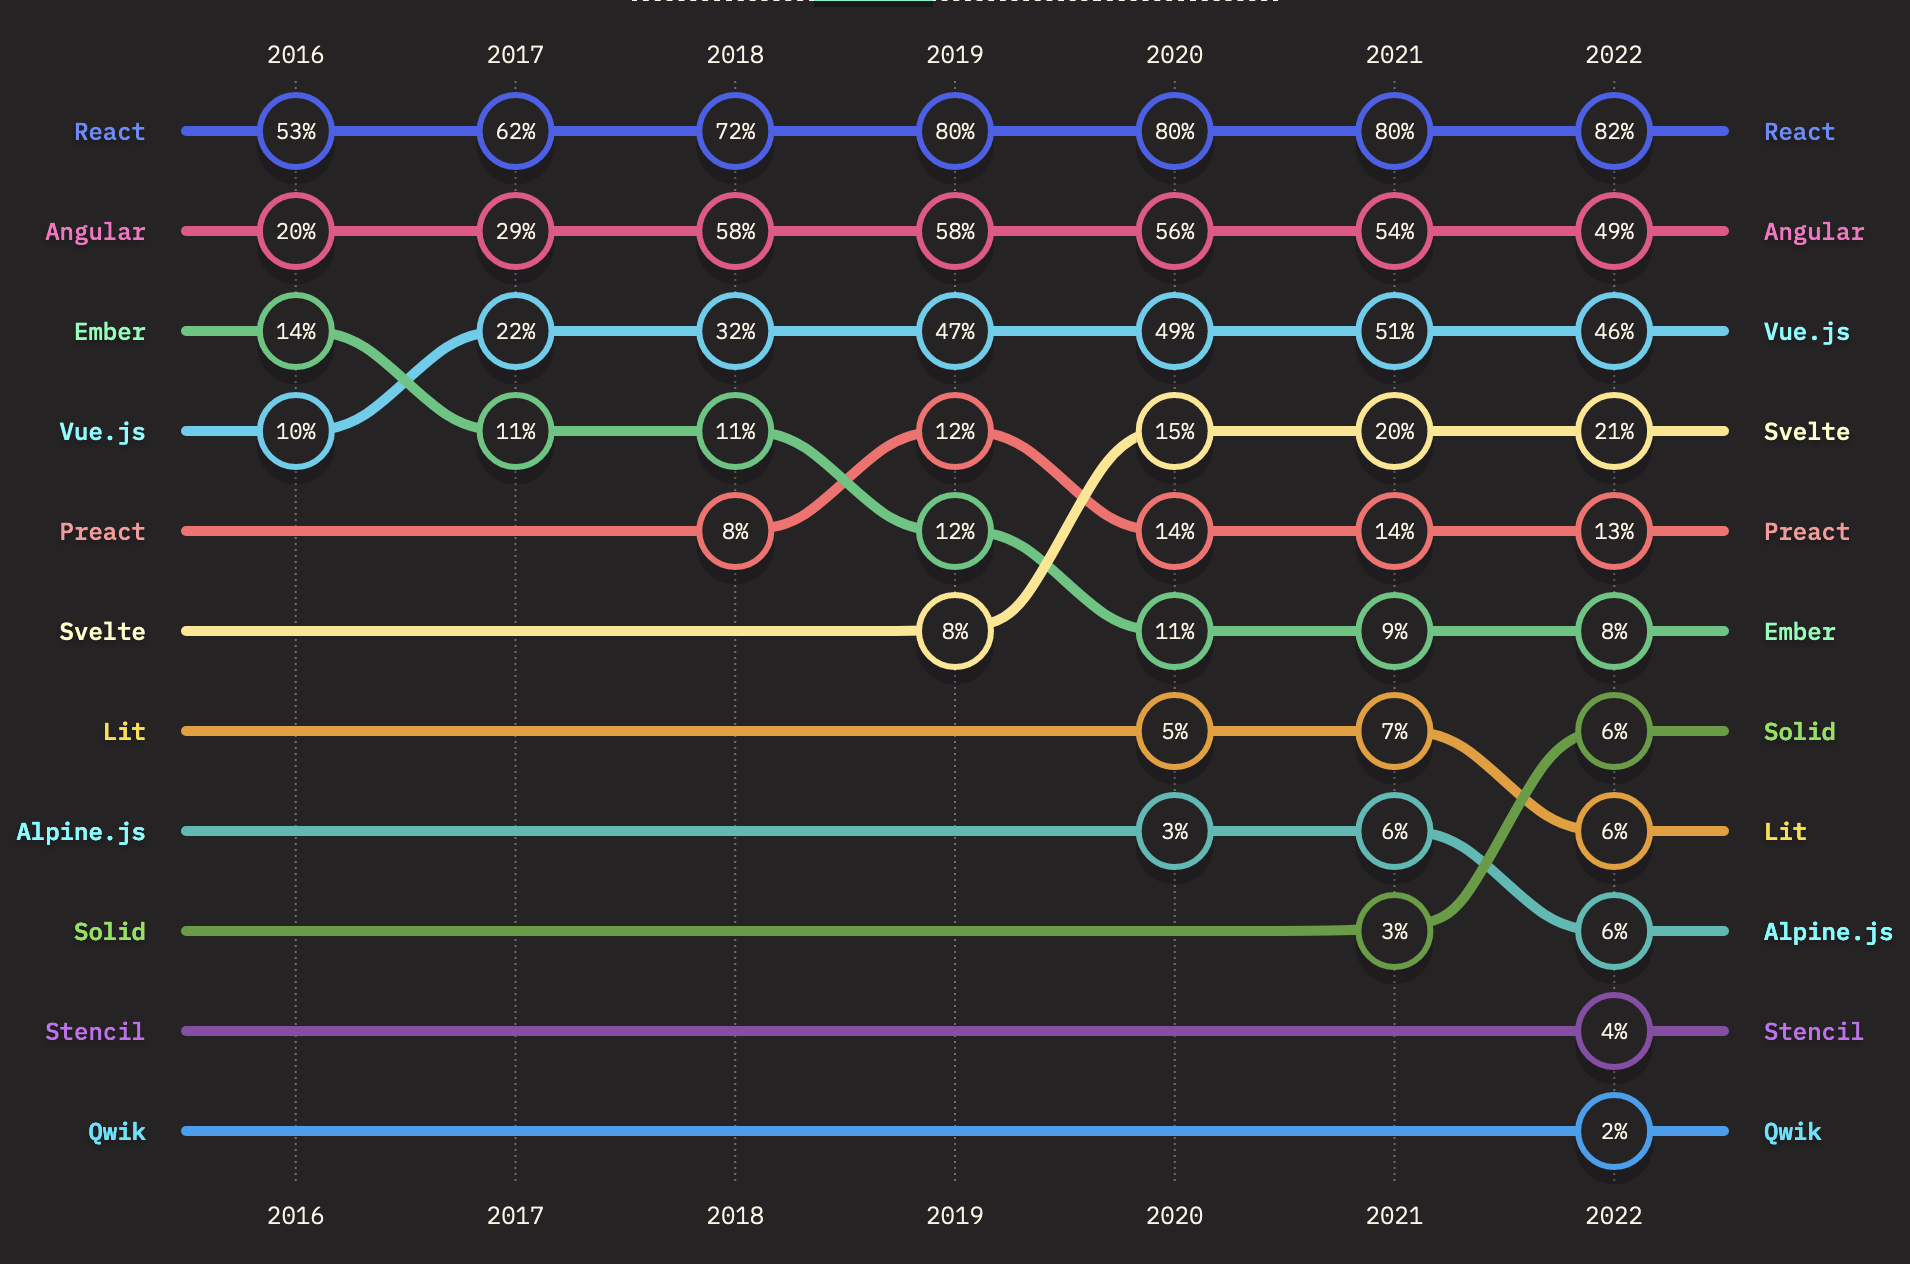
\includegraphics[scale=0.4]{04_Artefakte/01_Abbildungen/stateofjs-usage-frontend-frameworks-2022}
    \caption[{Most used frontend frameworks in 2022}]{State of JS: Most used frontend frameworks in 2022\protect\footnotemark}
    \label{fig:mostUsedFrameworks}
\end{figure}
\footnotetext{\cite{mostUsedFrontendFrameworks22}}

\subsection{React}

\emph{React} (\url{https://react.dev/}), developed by \emph{Facebook} and maintained by its successor \emph{Meta}, has become the most widely used tool for building \ac{SPA}s and is steadily leading the rankings for most used frontend frameworks both in the \emph{StackOverflow} \parencite{stackOverflowPollWebFrameworks23} and the \emph{State Of JS} \parencite{mostUsedFrontendFrameworks22} polls. By definition, it is not a framework but a \ac{UI} library that builds on other extensions to support state management, routing and deployment functionality. Although it is not a framework itself, there are existing frameworks like \emph{Next.js} (\url{https://nextjs.org/}) for the web and \emph{ReactNative} (\url{https://reactnative.dev/}) for building mobile apps using native functionality. React makes use of \ac{JSX}, which allows directly mixing inline \ac{HTML} with the \ac{JS} or \ac{TS} code structure.

\subsection{Vue.js}

\emph{Vue.js} (\url{https://vuejs.org/}) was developed by Evan You and is maintained by an international team of individuals. It had a relatively marginal presence in the first years after its inception. This can be partially attributed to its origin in China, and most of its supporting modules were localised in Chinese. Over the years, it grew in popularity and received much more international support, eventually overcoming the language barrier. Unlike \emph{React}, it is billed as a "progressive framework" that provides fundamental functionality for building reactive components but also accommodates more complex use-cases \parencite{vueProgressiveFramework}. \emph{Vue.js} builds on standard \ac{JS} or \ac{TS}, \ac{HTML} and \ac{CSS} to build components, recommending a simple template mechanism mixed with reactive substitutions. However, it also supports using \ac{JSX} for specifying inline \ac{HTML} within \ac{JS}. As with \emph{React}, there are extensions and frameworks like \emph{Quasar} (\url{https://quasar.dev/}) and \emph{Nuxt} (\url{https://nuxt.com/}) that enable even more sophisticated workflows for application development and deployment.

\subsection{Angular}

\emph{Angular} was initially released by \emph{Google} in 2010 as \emph{AngularJS}  and officially discontinued in 2022 (\url{https://angularjs.org/}). A completely overhauled and currently used version 2 was released in 2016 and maintained by \emph{Google}. It is different from \emph{React} and \emph{Vue.js} in that it is a complete framework that contains everything required to build and deploy an application, and it explicitly recommends \ac{TS} as a programming language. The framework is also less flexible in that it is opinionated and has its own set of best practices baked into the framework's structure.




\section{Backend Libraries}

\subsection{Express}

\subsection{Koa}

\subsection{Fastify}


\section{Backend Frameworks}

\subsection{Nest JS}

\subsection{Meteor}

\subsection{Feathers}

